
		%\title{Answer to Reviewer #1}
		%\maketitle
		
%		\begin{letter}{}
%
%		\opening{Answer to Reviewer \#2}
		%	\opening{Dear Prof. Roman Slowinski\\Coordinating Editor of EJOR}
		
		\section*{Answer to reviewer \# 2}
		Thanks a lot for dedicating your time to revise our work. We found every one of your comments very helpful and insightful, and we believe that after taking them into account our work has much improved.
		
		Following we provide replies to each one of the comments you have given us:
		
		\textbf{Comment \#1:} ``The highlights (contributions of the paper) and organization of the remaining sections should be presented at the end of Section 1."
		\\
		
		We addressed this issued by adding a paragraph to the end of our Introduction:
		
		``This paper is organized as follows. Section 2 presents the definitions of both problems and introduces some notations used throughout the rest of the work. An algorithm for MCE is developed
		in Section 3, and an algorithm for MCER in Section 5 with the observation that its development
		depends on a subproblem whose algorithm is developed in Section 4. Improvements suggestions to
		the implementations are given in Section 6 while the implementation details are given in Section 7.
		Numerical results are presented and analyzed in Section 8. Finally, a conclusion is given in Section 9."
		
		This paragraph can be found in the manuscript in pages 3 and 4.
		\\
		
		\textbf{Comment \#2:} ``In my opinion `fixed shape' ellipses should be replaced by `fixed shape parameters' ellipses, or ellipses with the given semi-major and semi-minor axes. Alternately the term `fixed shape' ellipses should be explained."
		\\
		
		Thanks for the great observation; we agree that it is not very clear what the term `fixed shape' ellipses means, and decided to rewrite the text everywhere it appeared. Please find below the changes we have made:
		\begin{itemize}
			\item In the first paragraph of the abstract (page 2), we used the term ``given their major and minor axis" to better convey the same idea.
			
			\item In the Introduction section (page 3), we changed the description of our problem to: ``(...) each ellipse is defined to have fixed major and minor axis and an undefined location (...)."
			
			\item Section 4 had in its title (page 7) ``(...) of An Ellipse Given Its Shape and (...)", we replaced it by ``(...) of An Ellipse Given Its Shape Parameters and (...)."
		\end{itemize}
		
		\textbf{Comment \#3:} ``Please, extend the description of practical applications."
		
		Thanks for the comment, we addressed this issued by adding a new paragraph to our Introduction citing the work ``\textit{Mustafa S. Canbolat and Michael von Massow. Planar maximal covering with ellipses.}", which covers with great detail the practical applications of the problems studied in our work:
		\\
		
		``In the real world, this problem comes up when a telecommunications company has to buy and
		place antennas over a region to distribute a signal to a population, not necessarily everyone, aiming
		profit maximization. More details about the applications of PMCLP can be found in [5], which also
		ponders about the practical importance of considering the PMCLP with elliptical coverage."
		
		This change can be found in page 3 of the manuscript. Also, to better fit this addition, we had to modify the paragraph after the added one; we do not display it here because it is not relevant to this comment.
		\\
		
		\textbf{Comment \#4:} ``The literature review in Introduction is a bit limited and should to be extended analyzing more approaches and references on the subject. It can be expected that beginning from the first publication [8] in 1984 a reasonable number of references on the subject have been published. See, e.g. papers:
		
		`A Combinatorial Maximum Cover Approach to 2D Translational Geometric Covering' by K. Daniels A. Mathur R. Grinde
		
		`Covering a polygonal region by rectangles' by G. Scheithauer, Y. Stoyan, T. Romanova, A. Krivulya
		
		`Translational polygon containment and minimal enclosure' using mathematical programming
		by V.J. Milenkovic , K. Daniels
		
		and references in 2007 PhD thesis of Daoqin Tong from the Ohio State University."
		\\
		
		Thanks for all the great suggestions, after pondering about it, we agree that our literature review needed work, it is great that you pointed it out.
		We spent some time on trying to improve it, and in summary, those are the changes we have made to our Introduction:

		\begin{itemize}
			\item We added a citation to ``H Younies and G O Wesolowsky. Planar maximal covering location problem under block norm distance measure". This shows another example of versions of PMCLP other than the classical one using Euclidean norm.
			\item We added a citation to the survey paper: ``Alan T. Murray. Maximal coverage location problem: Impacts, significance, and evolution.". Instead of giving an extensive review, we use a common practice of citing a survey paper. 
		\end{itemize}
	
	After these additions, the piece of our Introduction doing literature review of PMCLP is as follows:
	
	``A continuous extension of MCLP, where the facility and demand sets are located on the plane and coverage is determined by a norm function, was introduced in [8] and named Planar Maximal	Covering Location Problem (PMCLP) following the advances on covering location problems on the	plane that were being made at the time.
	
	PMCLP can be seen as a class of problems, as, in general, facilities can have their coverage
	defined by any norm function, and the demand set, although initially defined as points, could have a more generic definition; in [4], for example, the demand set is defined as a set of rectangles; and in [20], a version of PMCLP where coverage is determined using block norms is studied. For a more comprehensive review on PMCLP and MCLP, please see [15].
	
	In our work, because of the similarities with the problems studied by us, we are particularly interested in the Euclidean PMCLP defined with coverage being determined by the Euclidean norm.	In [8], a method for this version of PMCLP was developed following the demonstration of a theorem,	which showed that a finite set of locations could be constructed to contain at least one optimal	solution transforming PMCLP into a combinatorial optimization problem."
	
	We did consider the list of works you gave us as suggestions, however, even though we think they are great papers, we decided to cite works that we judged to be closer to the problems we are studying. We also had the goal to not extend the literature review too much, as the field of geometric covering is too vast, we tried to keep it concise by only citing works that study very specific problems, and a survey paper.
	It is worth mentioning though, that some works of Daoqin Tong are cited in the survey paper we are using. If after reading this, you still feel like our literature review is not satisfactory, we can change it to include your suggestions.
\\
	
		\textbf{Comment \#5:} ``Please, clarify what is the critical parameter for your algorithm: the number of ellipses or the number of demand points?"
		\\
		
		We addressed this issue in Section 8.2 ``New instances" (page 19):
		
		``We were able to run experiments with up to 700 demand points; however, it is clear that the number of ellipses is the critical parameter of both algorithms, as even for small demand sets, we could not go over 7 ellipses."
		\\
		
		\textbf{Comment \#6:} ``In the paper overlapping of covering ellipses is allowed, i.e. a demand point can be covered by more than one ellipse. However, it seems natural that the weight of the demand point covered by various ellipses can differ from the weight of the same point covered by only one ellipse."
		\\
		
		Thanks for this comment, we, too, think that depending on the viewpoint, considering the weight of each point to be a function which depends on the set of ellipses covering it is more natural. We believe that our methods could be trivially adapted to work with this different definition, however, we also think that we have to ponder about doing this change because this is not the traditional definition of any other PMCLP we have based our developments on; meaning that we would have to have a strong motive for this not to look like an arbitrary change.
		\\	
		
		\textbf{Comment \#7:} ``What happens if no overlapping between covering ellipses is allowed. Please, comment on this."
		\\
		
		Thanks for the great question, we thought a lot about this, and we came up with some arguments to show you what happens if we add this constraint to our problem.
		
		First, for an example of covering without overlapping, please see the paper ``Covering point sets with two disjoint disks or squares" by Cabello, S., Díaz Báñez, J.M., Seara, C., Sellarès, J.A., Urrutia, J., Ventura, I.
		
		This work deals with the problem of covering points using two Euclidean disks with the constraint of no overlapping being allowed. This article is cited by a work we are citing in our Introduction: ``Covering many or few points with unit disks." by Mark de Berg, Sergio Cabello, and Sariel Har-Peled. 
		This work develops an algorithm for the overlap-allowed covering of points by multiple Euclidean disks. In its Introduction, the authors cite the previous work that does not allow overlap saying: ``This condition changes the problem significantly, because now issues related to packing problems arise". 
		Based on this, we are safe to say that we should expect that adding a no-overlap constraint would change our problem significantly too.
		
		We also produced an example to show you what would happen if we simply added this constraint without changing anything to our method. 
		The way our algorithms work is that it looks for solutions with points on the ellipses. This type of solution is not favorable when we have this constraint as, for example, see the counter-example in this figure:  

		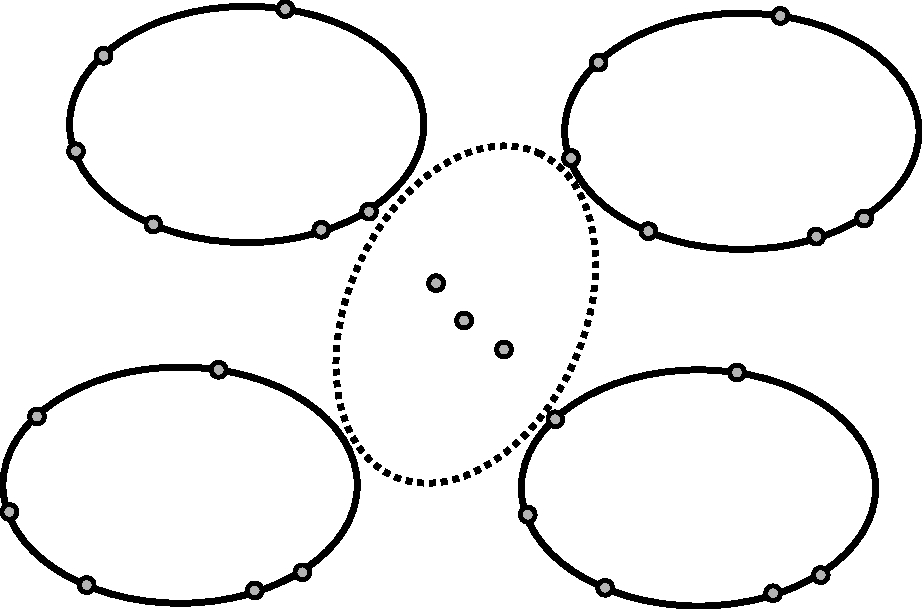
\includegraphics[scale=.6]{figures/answer-to-reviewer-2}

		The solution shown is non-overlapping -- actually there are an infinite number of non-overlapping equivalent solutions. However, our algorithm would fail to find any equivalent solution. Notice that moving the ellipse with no points on its coverage region's border in order to put at least two points on it would cause overlap.
		We believe methods for the problems with this additional constraint would have to come from a different basis.
		
		
	%	\closing{On behalf of the authors and with our best regards,}
	%		\end{letter}